\documentclass[tikz,border=2pt]{standalone}
\usepackage{amsmath,amssymb}
\usepackage{tikz}

\begin{document}
% Silver-Meal: extend the coverage of the order placed in period i while the average cost
% per covered period TCU(i,t) decreases; stop at the first local minimum (illustrative values).
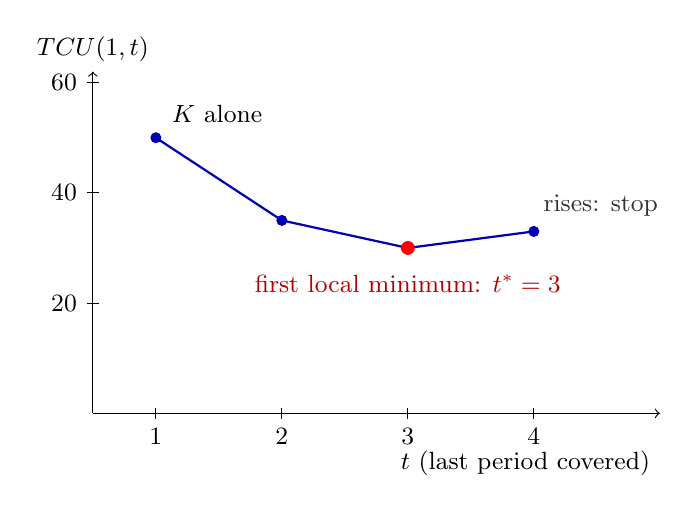
\begin{tikzpicture}[every node/.style={font=\small}, x=1.6cm, y=0.07cm]
	\draw[->] (0.5,0) -- (5.0,0);
	\node[anchor=north east] at (5.0,-5) {$t$ (last period covered)};
	\draw[->] (0.5,0) -- (0.5,62) node[above] {$TCU(1,t)$};
	\foreach \t in {1,2,3,4} {\draw (\t,1) -- (\t,-1) node[below] {$\t$};}
	\foreach \c in {20,40,60} {\draw (0.55,\c) -- (0.45,\c) node[left] {$\c$};}
	\draw[blue!70!black, thick] (1,50) -- (2,35) -- (3,30) -- (4,33);
	\fill[blue!70!black] (1,50) circle (2pt); \fill[blue!70!black] (2,35) circle (2pt); \fill[red] (3,30) circle (2.5pt); \fill[blue!70!black] (4,33) circle (2pt);
	\node[anchor=south west] at (1.05,51) {$K$ alone};
	\node[red!70!black, anchor=north] at (3,27) {first local minimum: $t^\ast=3$};
	\node[gray!40!black, anchor=south west] at (4.0,34) {rises: stop};
	\end{tikzpicture}
\end{document}
